\chapter{}
\section{}
Es soll anhand der Angaben auf dem Leistungsschild die Polpaarzahl der Asynchronmaschine bestimmt werden. Dazu sollen nun Überlegungen angestellt werden. Auf dem Typenschild finden sich Angaben über die Nenndrehzahl N, die Frequenz f. Mit diesen Daten kann die Polpaarzahl näherungsweise bestimmt werden.
\begin{equation}
	Z_{P} = 60\frac{f}{N}
\end{equation}
Der Faktor 60 kommt daher zustande, da die Drehzahl von $ s^{-1} $ in $ min^{-1} $ umgerechnet werden muss. Die Asynchronmaschine weist einen Schlupf auf, ohne diesen würde sie gebremst werden. Aufgrund dieses Schlupfes ist die Drehzahl auf dem Typenschild geringer als die Drehfelddrehzahl. Deshalb erhalten wir keinen ganzzahligen Wert für die  Polpaarzahl. Das ist jedoch unzulässig, da es nur ganzzahlige Werte geben darf, weshalb hier auf die nächste ganzzahlige Anzahl abgerundet wird.

\section{}
Anhand der zuvor getroffenen Überlegungen soll nun die Polpaarzahl der im Labor befindlichen Asynchronmaschine bestimmt werden. Auf dem Leistungsschild unseres Motors befinden sich folgende Angaben über die Frequenz des Motors, sowie zu dessen Nenndrehzahl:
\begin{center}
	$ f = 50Hz $ \hspace{2cm} $ N = 1370min^{-1} $
\end{center}
Somit ergibt sich folgende Polpaarzahl:
\begin{equation}
	Z_{P} = 60\frac{50Hz}{1370min^{-1}} = 2.19 \approx 2
\end{equation}

\section{}
\begin{figure}[h]
	\centering
	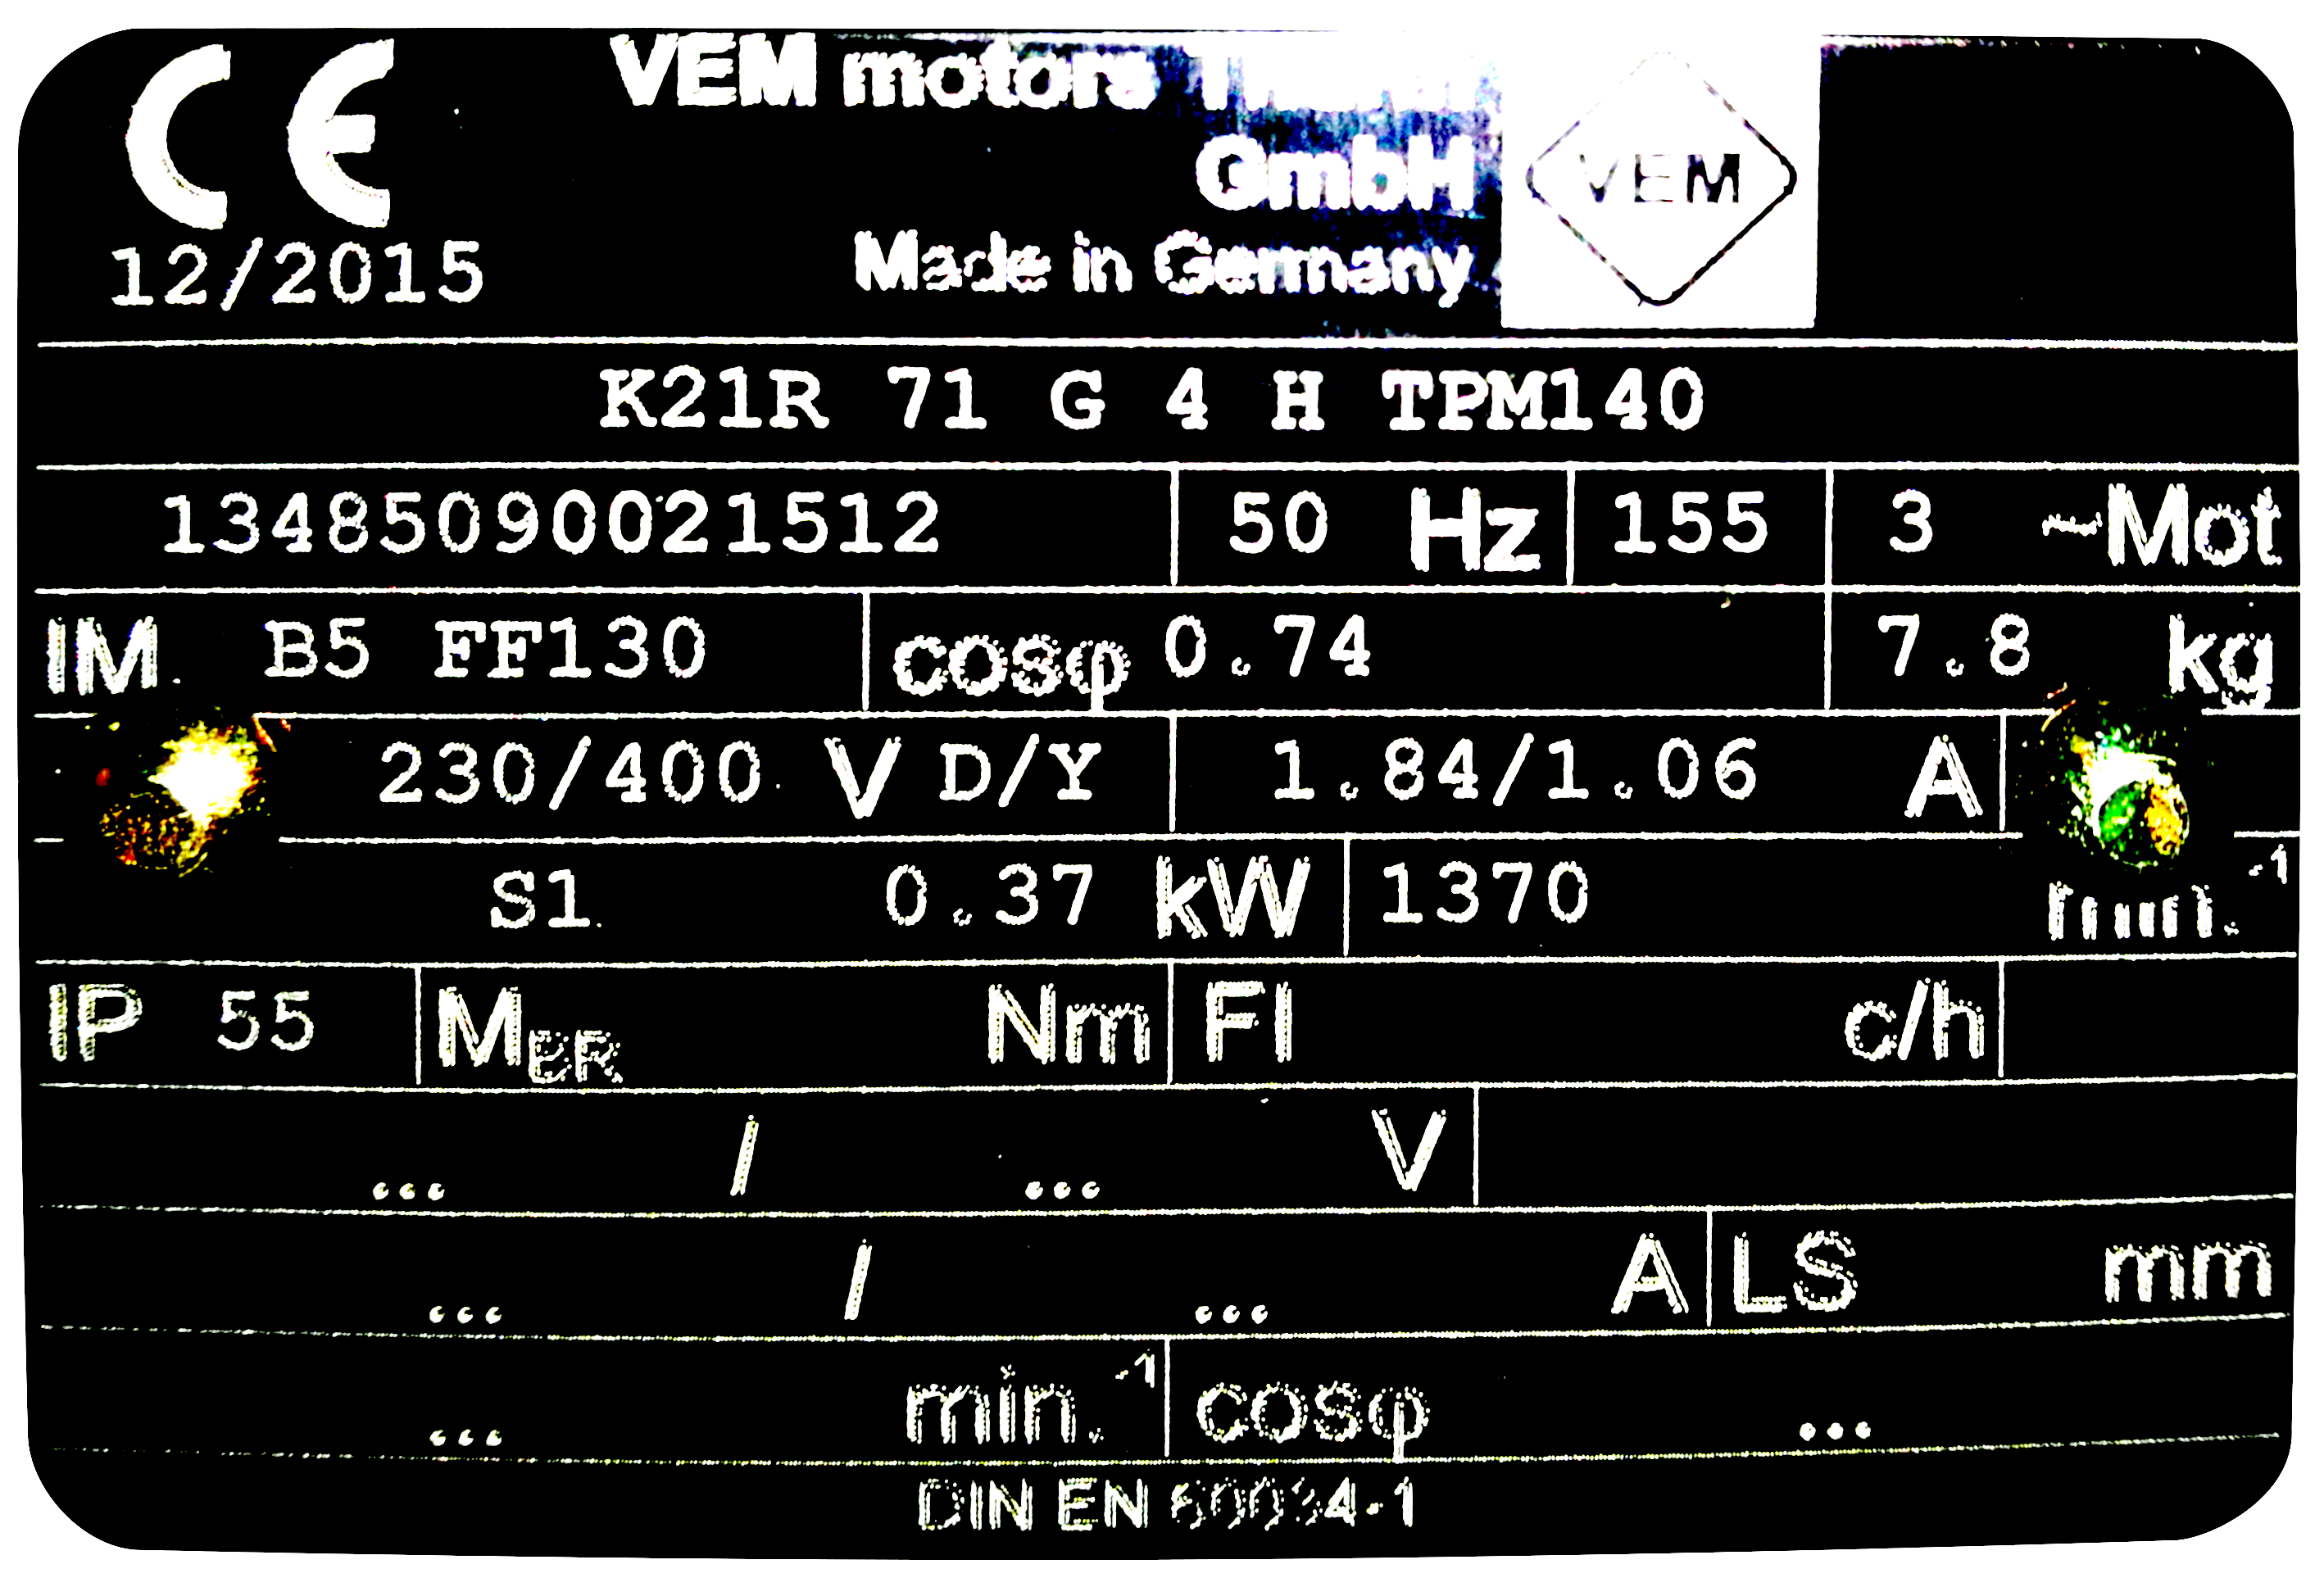
\includegraphics[width=0.6\textwidth]{./Bilder/Typenschild.png}
	\caption{Leistungsschild der Asynchronmaschine}
	\label{fig:4c:typenschild}
\end{figure}